% generated by report/gen_tables.py from build/scene_export.json -- do not edit
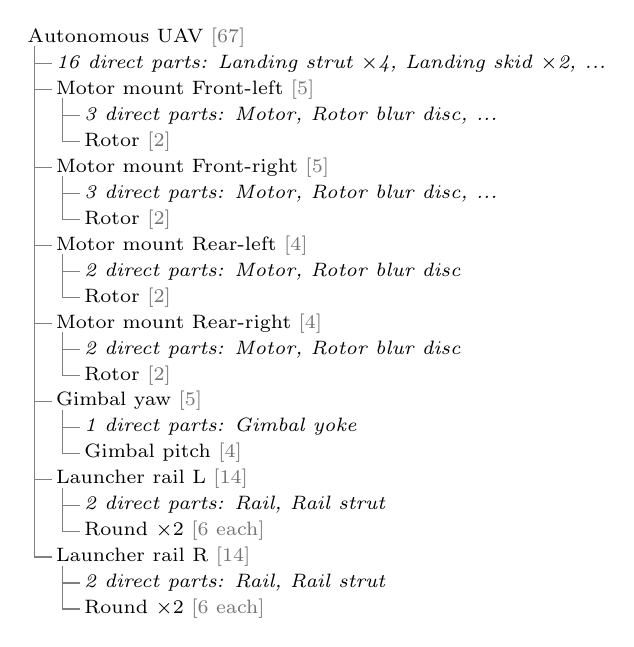
\begin{tikzpicture}[x=0.36cm,y=-0.33cm,font=\scriptsize]
\node[anchor=west,inner sep=0pt] (n0) at (0,0) {Autonomous UAV \textcolor{black!55}{[67]}};
\node[anchor=west,inner sep=0pt] (n1) at (1,1) {\textit{16 direct parts: Landing strut $\times$4, Landing skid $\times$2, ...}};
\draw[black!50,thin] (0.25,0.35) |- (0.88,1);
\node[anchor=west,inner sep=0pt] (n2) at (1,2) {Motor mount Front-left \textcolor{black!55}{[5]}};
\draw[black!50,thin] (0.25,0.35) |- (0.88,2);
\node[anchor=west,inner sep=0pt] (n3) at (2,3) {\textit{3 direct parts: Motor, Rotor blur disc, ...}};
\draw[black!50,thin] (1.25,2.35) |- (1.88,3);
\node[anchor=west,inner sep=0pt] (n4) at (2,4) {Rotor \textcolor{black!55}{[2]}};
\draw[black!50,thin] (1.25,2.35) |- (1.88,4);
\node[anchor=west,inner sep=0pt] (n5) at (1,5) {Motor mount Front-right \textcolor{black!55}{[5]}};
\draw[black!50,thin] (0.25,0.35) |- (0.88,5);
\node[anchor=west,inner sep=0pt] (n6) at (2,6) {\textit{3 direct parts: Motor, Rotor blur disc, ...}};
\draw[black!50,thin] (1.25,5.35) |- (1.88,6);
\node[anchor=west,inner sep=0pt] (n7) at (2,7) {Rotor \textcolor{black!55}{[2]}};
\draw[black!50,thin] (1.25,5.35) |- (1.88,7);
\node[anchor=west,inner sep=0pt] (n8) at (1,8) {Motor mount Rear-left \textcolor{black!55}{[4]}};
\draw[black!50,thin] (0.25,0.35) |- (0.88,8);
\node[anchor=west,inner sep=0pt] (n9) at (2,9) {\textit{2 direct parts: Motor, Rotor blur disc}};
\draw[black!50,thin] (1.25,8.35) |- (1.88,9);
\node[anchor=west,inner sep=0pt] (n10) at (2,10) {Rotor \textcolor{black!55}{[2]}};
\draw[black!50,thin] (1.25,8.35) |- (1.88,10);
\node[anchor=west,inner sep=0pt] (n11) at (1,11) {Motor mount Rear-right \textcolor{black!55}{[4]}};
\draw[black!50,thin] (0.25,0.35) |- (0.88,11);
\node[anchor=west,inner sep=0pt] (n12) at (2,12) {\textit{2 direct parts: Motor, Rotor blur disc}};
\draw[black!50,thin] (1.25,11.35) |- (1.88,12);
\node[anchor=west,inner sep=0pt] (n13) at (2,13) {Rotor \textcolor{black!55}{[2]}};
\draw[black!50,thin] (1.25,11.35) |- (1.88,13);
\node[anchor=west,inner sep=0pt] (n14) at (1,14) {Gimbal yaw \textcolor{black!55}{[5]}};
\draw[black!50,thin] (0.25,0.35) |- (0.88,14);
\node[anchor=west,inner sep=0pt] (n15) at (2,15) {\textit{1 direct parts: Gimbal yoke}};
\draw[black!50,thin] (1.25,14.35) |- (1.88,15);
\node[anchor=west,inner sep=0pt] (n16) at (2,16) {Gimbal pitch \textcolor{black!55}{[4]}};
\draw[black!50,thin] (1.25,14.35) |- (1.88,16);
\node[anchor=west,inner sep=0pt] (n17) at (1,17) {Launcher rail L \textcolor{black!55}{[14]}};
\draw[black!50,thin] (0.25,0.35) |- (0.88,17);
\node[anchor=west,inner sep=0pt] (n18) at (2,18) {\textit{2 direct parts: Rail, Rail strut}};
\draw[black!50,thin] (1.25,17.35) |- (1.88,18);
\node[anchor=west,inner sep=0pt] (n19) at (2,19) {Round $\times$2 \textcolor{black!55}{[6 each]}};
\draw[black!50,thin] (1.25,17.35) |- (1.88,19);
\node[anchor=west,inner sep=0pt] (n20) at (1,20) {Launcher rail R \textcolor{black!55}{[14]}};
\draw[black!50,thin] (0.25,0.35) |- (0.88,20);
\node[anchor=west,inner sep=0pt] (n21) at (2,21) {\textit{2 direct parts: Rail, Rail strut}};
\draw[black!50,thin] (1.25,20.35) |- (1.88,21);
\node[anchor=west,inner sep=0pt] (n22) at (2,22) {Round $\times$2 \textcolor{black!55}{[6 each]}};
\draw[black!50,thin] (1.25,20.35) |- (1.88,22);
\end{tikzpicture}
